\section{Introduction}
\label{sec:intro}

Difference-in-differences (DID) is a workhorse design across empirical economics,
and a particularly visible one in environmental policy---our motivating case.
Studies of carbon pricing, emissions-trading pilots, and industrial-emission
standards routinely compare treated and untreated units before and after a
policy to recover its causal effect. The credibility of any
such estimate rests entirely on a chain of \emph{identification assumptions}:
that treated and control units would have moved in parallel absent the policy,
that units did not anticipate it, that staggered adoption is handled with an
appropriate estimator, that there is no interference between treated and control
units, and so on. A decade of methodological work has shown how fragile each of
these assumptions can be, and how easily a standard two-way fixed-effects
specification can mislead under heterogeneous and staggered treatment timing
\cite{goodmanbacon2021,callaway2021,sunabraham2021,dechaisemartin2020,roth2023}.

Yet in applied work these assumptions are frequently \emph{asserted} rather than
\emph{audited}. A paper states that parallel trends ``hold'', shows an
event-study plot, and moves on; a reader who wants to know whether the
identification argument is actually supported by the reported evidence must
reconstruct it by hand, dimension by dimension. This is slow, expert-intensive,
and inconsistent across reviewers. The result is a reliability gap in a body of
evidence that increasingly informs environmental policy.

\paragraph{Our stance.}
We argue that identification \emph{credibility} is auditable even though the
causal \emph{effect} is not. In a DID design the counterfactual is never
observed, so it is hopeless---and, we contend, the wrong target---to ask an
automated system ``is the estimated effect true?''. Instead we ask a question
that can be grounded in the paper itself: \emph{is each identification assumption
supported by the evidence the study reports, and where is that support weakest?}
This reframing turns an unanswerable causal question into a tractable auditing
problem over assumptions, their testable implications, and the in-paper evidence
that bears on them. A useful system should therefore localize where support is
fragile rather than issue a verdict.

\paragraph{Why human calibration.}
Identification credibility is not a binary truth label. A dimension is rarely
simply ``satisfied'' or ``violated''; reviewers grade it on a severity scale, and
where the low/medium/high boundaries fall is a matter of expert judgement. Some
disagreement is therefore intrinsic---especially when a DID-specific check is
applied to a non-standard design, where the dimension may not apply as
conventionally defined. We treat this ambiguity as a feature of the task, not
noise: ARGUS pairs automated, evidence-grounded auditing with a
\emph{human-calibrated severity} scale, using a pilot expert gold both to
\emph{evaluate} the auditor and to \emph{calibrate} how severely it flags.

\paragraph{ARGUS.}
We introduce \textbf{ARGUS}, a responsible-AI framework that audits the
identification credibility of DID environmental-policy studies. ARGUS decomposes
identification into a fixed set of auditable dimensions, gathers the supporting
evidence each dimension requires, assesses every
assumption--implication--evidence chain, localizes risk across dimensions, and
produces a transparent, evidence-anchored report for a human expert
(Figure~\ref{fig:overview}). It is deliberately a \emph{bounded-agentic} system: the pipeline between modules is
fixed and deterministic, and model-driven agency is confined to two scoped
sub-tasks. Because the true effect is unavailable as ground truth, we validate
the auditor with \emph{synthetic flaw injection}: we perturb a credible paper
with one known identification flaw and check whether ARGUS detects it, stays
quiet on the clean version, and localizes the right dimension. The injected flaw
is local ground truth that requires no access to the true effect. Deploying ARGUS
on real papers then exposes \emph{evidence grounding}---retrieving the right
evidence---as the binding constraint, and a pilot human gold reveals a systematic
over-severity bias that a lightweight, anchor-based calibration layer reduces
while preserving high-risk recall. ARGUS is thus best read as a
\emph{high-sensitivity screening tool} that flags dimensions for expert
review---\emph{flag, not judge}---not an autonomous arbiter of causal truth.

\paragraph{Contributions.}
This paper, presented as a doctoral-research plan, makes four contributions.
\textbf{(i)}~a structured \textbf{11-dimension audit framework} for DID
identification credibility that targets \emph{reported-evidence adequacy} rather
than causal truth (\S\ref{sec:framework});
\textbf{(ii)}~a \textbf{bounded-agentic} evidence-retrieval and assessment
pipeline, with model agency confined to two scoped, traceable sub-tasks behind a
fixed deterministic control flow;
\textbf{(iii)}~a \textbf{multi-stage evaluation}---synthetic flaw injection (where
adequacy reasoning lifts detection from a keyword baseline's $0.18$ to $1.0$) and
real-paper deployment on 27 DID papers, which relocates the bottleneck from
adequacy reasoning to \emph{evidence grounding} (\S\ref{sec:results}); and
\textbf{(iv)}~a \textbf{pilot human-gold calibration loop} (5 papers, 55
dimension-level cells): comparing ARGUS to an adjudicated gold reveals a
one-directional over-severity bias (more severe than gold in 28/33 answered cells,
less severe in none), and a lightweight calibration layer keyed on human anchors
reduces it while preserving high-risk recall---showing that expert annotation can
not only \emph{evaluate} but \emph{calibrate} an identification audit. The
human-gold analysis is pilot-scale; larger expert-labelled corpora are future
work.

\begin{figure}[t]
  \centering
  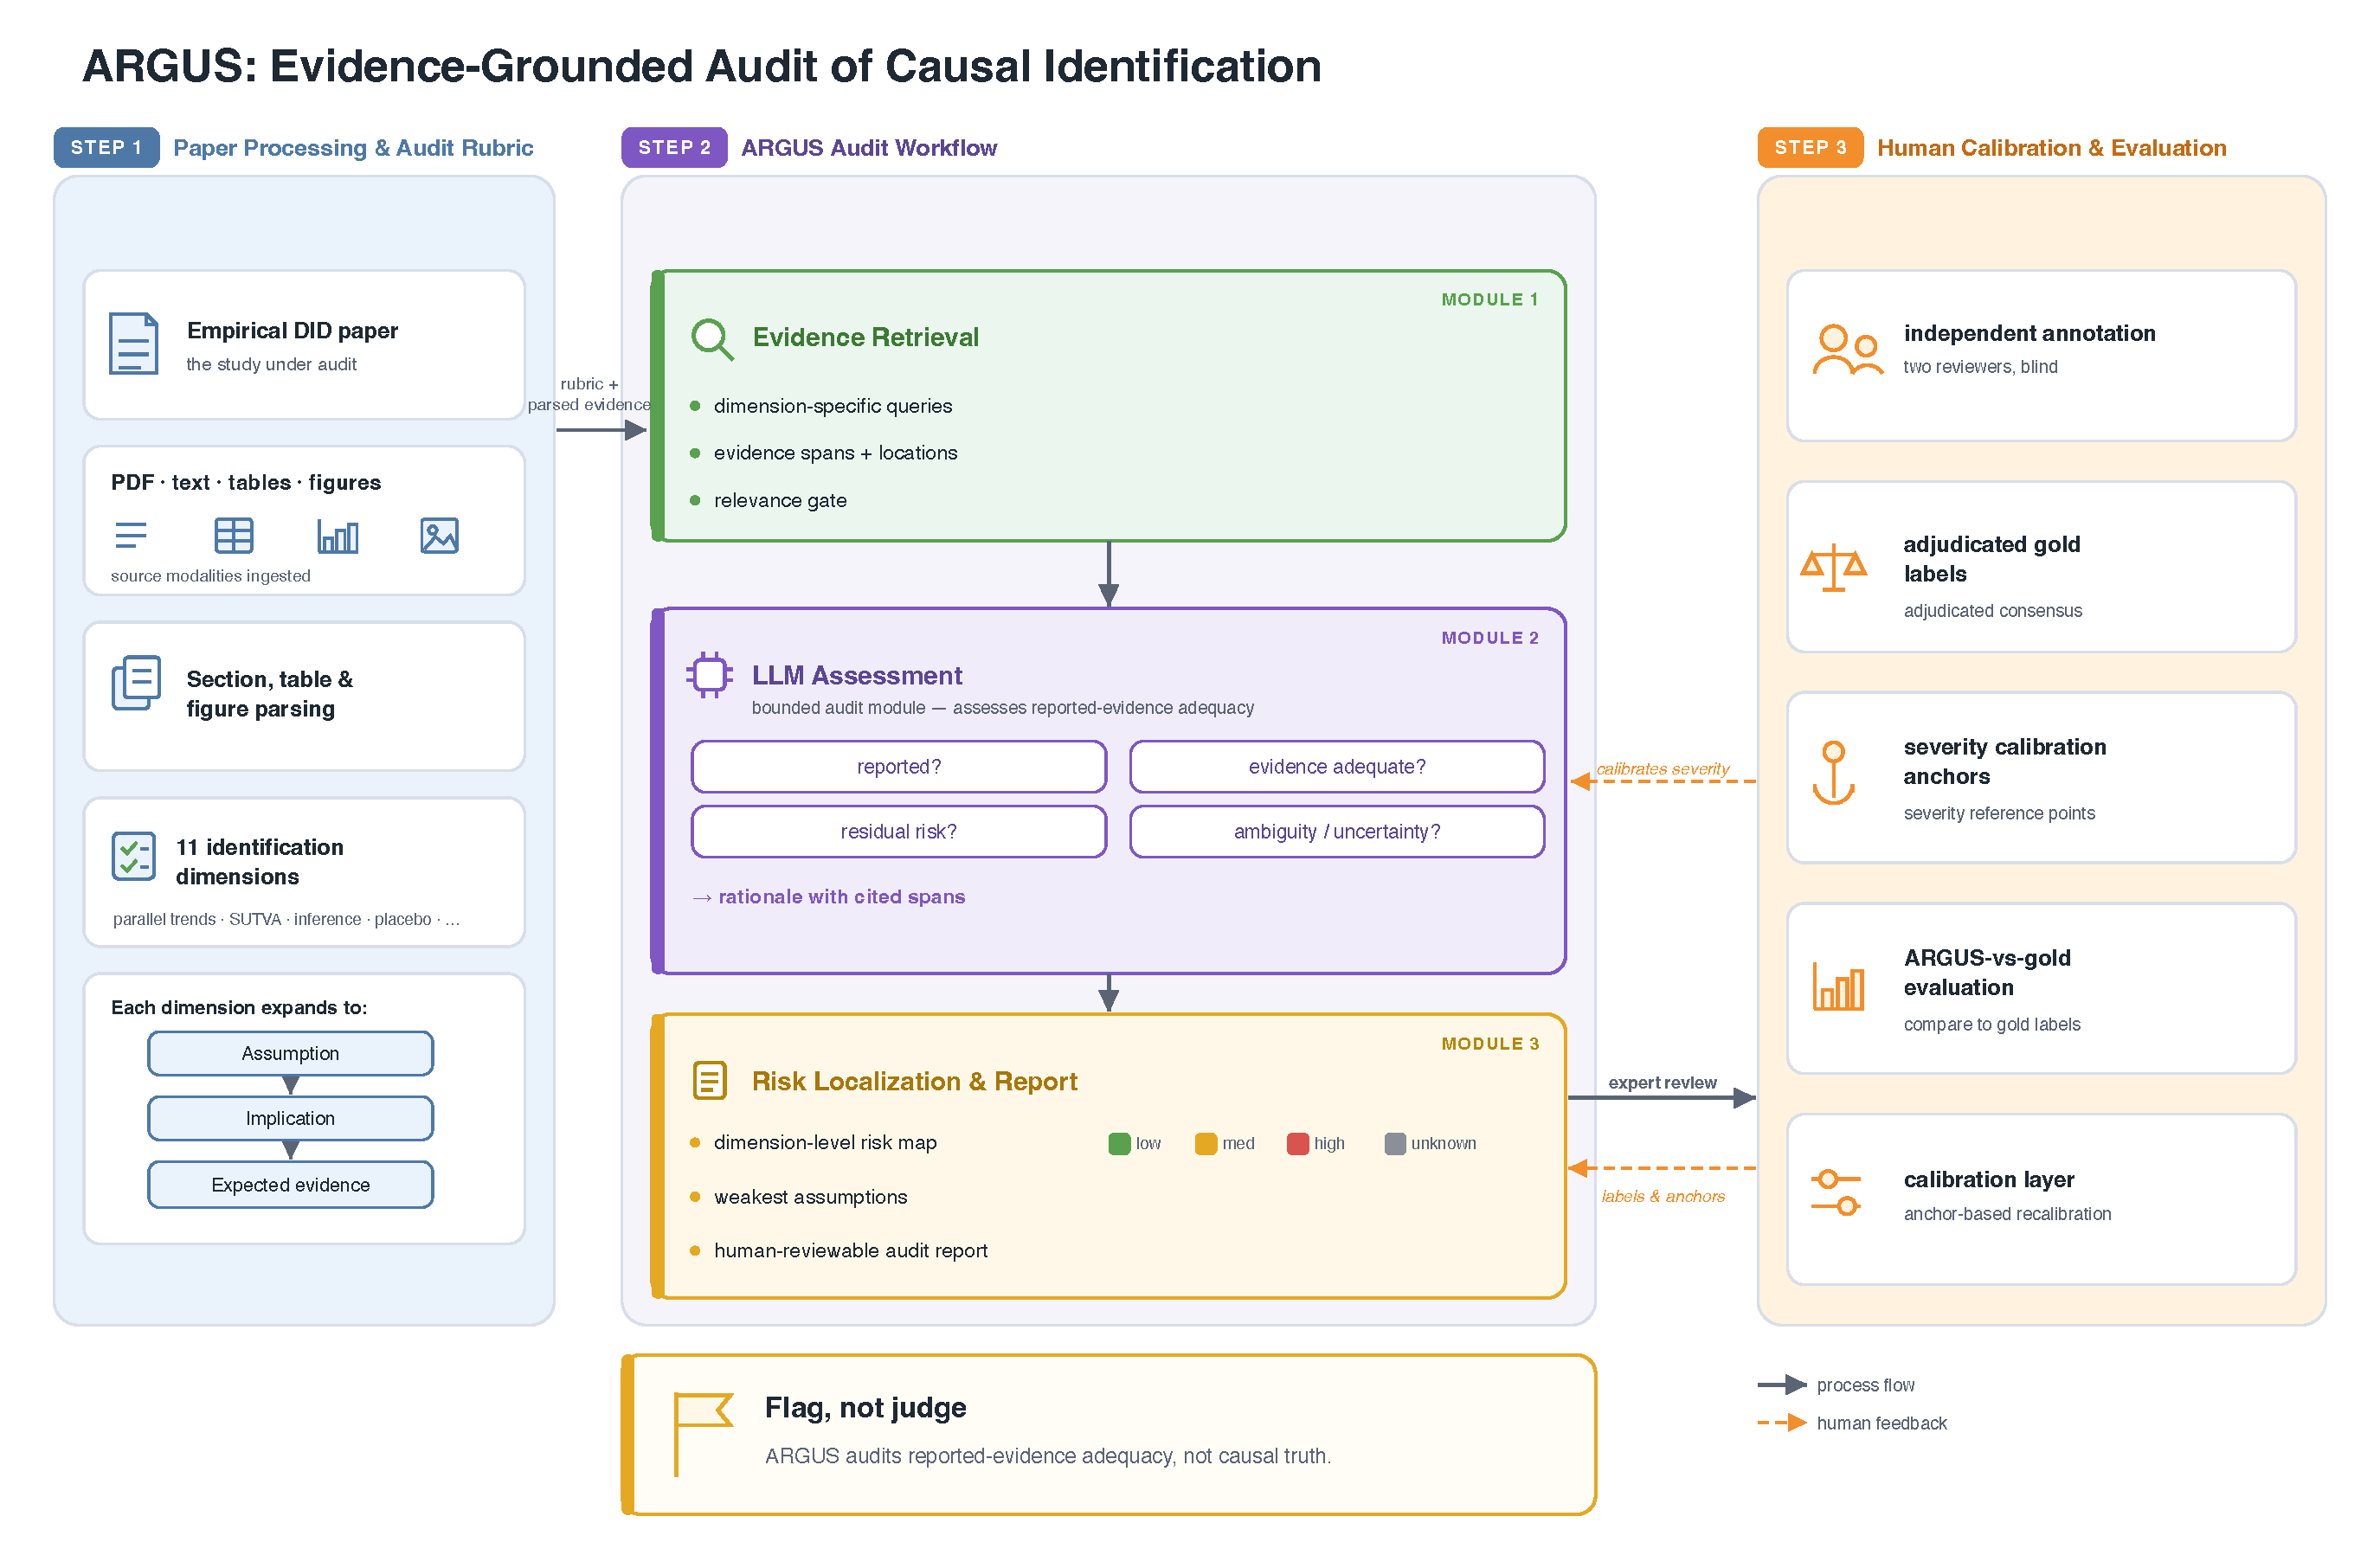
\includegraphics[width=\textwidth]{figures/argus_framework_simplified}
  \caption{Overview of ARGUS. Given an empirical DID paper, ARGUS retrieves
  dimension-specific evidence, assesses whether the reported evidence supports the
  relevant identification assumptions, and produces a human-reviewable risk
  report. A human calibration loop provides adjudicated gold labels and severity
  anchors for evaluating and calibrating the audit system. ARGUS is intended to
  flag dimensions for expert review, not to adjudicate causal truth.}
  \label{fig:overview}
\end{figure}
